%                                                                 aa.dem
% AA vers. 9.1, LaTeX class for Astronomy & Astrophysics
% demonstration file
%                                                       (c) EDP Sciences
%-----------------------------------------------------------------------
%
% \documentclass[referee]{aa} % for a referee version
%\documentclass[onecolumn]{aa} % for a paper on 1 column  
%\documentclass[longauth]{aa} % for the long lists of affiliations 
%\documentclass[letter]{aa} % for the letters 
%\documentclass[bibyear]{aa} % if the references are not structured 
%                              according to the author-year natbib style

%

\documentclass{aa}  

%
\usepackage{graphicx}
\usepackage{amsmath,amsfonts,amssymb}
\usepackage{natbib}


%%%%%%%%%%%%%%%%%%%%%%%%%%%%%%%%%%%%%%%%
\usepackage{txfonts}
\usepackage{xcolor}

\usepackage{blindtext}
%%%%%%%%%%%%%%%%%%%%%%%%%%%%%%%%%%%%%%%%
% \usepackage[options]{hyperref}
% To add links in your PDF file, use the package "hyperref"
% with options according to your LaTeX or PDFLaTeX drivers.
\usepackage{float}
%\usepackage{stfloats}
\usepackage{dblfloatfix}
\usepackage{afterpage}
\usepackage{ifthen}
\usepackage[morefloats=12]{morefloats}

\usepackage{placeins}
\usepackage{multicol}
%\usepackage[breaklinks,colorlinks,citecolor=blue]{hyperref}
\bibpunct{(}{)}{;}{a}{}{,}
\usepackage[switch]{lineno}
\definecolor{linkcolor}{rgb}{0.6,0,0}
\definecolor{citecolor}{rgb}{0,0,0.75}
\definecolor{urlcolor}{rgb}{0.12,0.46,0.7}
\usepackage[breaklinks, colorlinks, urlcolor=urlcolor,
    linkcolor=linkcolor,citecolor=citecolor,pdfencoding=auto]{hyperref}
\hypersetup{linktocpage}
\usepackage{bold-extra}

%Planck style file, to be used with A&A style to produce Planck papers for publication.
%
% version 28 September 2010 --- useful macros --- CRL
% version 17 October 2010   --- first cut at important instrument values, from Daniele Mennella and
%                               Francois Bouchet, 13 October 2010 --- CRL
% version 18 October 2010   --- LFI FWHM changed to one value per feed, rather than M & S separately
%                               LFI FWHM uncertainties added for individual feeds.  Corrections made
%                               to LFI values. --- Andrea Zacchei
% version 24 October 2010   --- added to and corrected definitions.  No changes made to instrument
%                               quantities. --- CRL 
% version 31 October 2010   --- added definition of \muKHz. --- CRL
%
% version 15 November 2010  --- fixed conflict with aa.cls in definition of \endtable
%                               by naming the command below "\endPlancktable".  See section
%                               13.16 of the Style Guide.
%
% version 06 December 2010  --- Set up names with and without units.
%                               Add \allearlypapers command to ensure that all early papers are
%                               included in the reference list.
%                               Define macro for the name of the 4He JT cooler.
%
% version 07 December 2010  --- removed extraneous "planck2011-1.2" entry in \allearlypapers
%
% version 12 December 2010  --- added \endPlancktablewide command to set tablenotes to the full
%                               page width in the \begin{table*}...\end{table*} environment when
%                               the ``twocolumn'' option is specified in the \documentclass command.
%                               (It would be more elegant to extract the appropriate width from the
%                               aa.cls system at the time of execution, but that is buried more
%                               deeply in the system than I investigated.)
%
% version 05 January 2011   --- added unit \MJysr.  HFI performance values updated per FRB email
%                               01/05/2011 02:38-0800, and Brendan Crill email 01/05/2011 18:08 -0800.
%
% version 06 January 2011   --- changed \scriptscriptstyle primes to \scriptstyle, to better match the
%                               tx fonts used by A&A.
%
% version 07 January 2011   --- modified \allearlypapers to correspond with final early paper list.  
%                               Fixed 545 GHz center frequency.
%
% version 07 January 2011b  --- changed LFI white-noise sensitivity numbers to correct problem with units
%
% version 05 July 2011      --- added \Msol and \Lsol to get the symbols for solar mass and luminosity.
%                               Deleted previous definitions of \solar and \sol, which were equivalent
%                               to the new \Msol.
%
% version 16 August 2011    --- changed comments on \endPlancktable and \endPlancktablewide for clarity
%
% version 11 September 2011 --- changed definition of \tablenote to make footnote labels italic, as per A\&A
%
% version 26 April 2011     --- changed definition of \Planck to agree with what is said in the Style Guide (!)
%
% version 04 Dec 2013       --- included 2013 results references
%
% version 17 Jan 2014       --- included fix to bibtex file v4.3, i.e. \providecommand{\sorthelp}[1]{}
%
% version 26 Jul 2014       --- fixed incompatibility problem with aa.cls v8.0 and v8.2.  v8.2 should now be used
%                               for all Planck papers.
%                           --- fixed problem in definition of "\all2013resultspapers" that introduced a blanck
%                               into the reference to p06b.
%                           --- removed all the parameter definition stuff at the end.  We weren't using it, and
%                               it took up a lot of space.
%
% version 28 Jan 2015       --- added "\alltwentyfiftennresultspapers" and corrected "\all2013resultspapers" to
%                               "\all20thirteenresultspapers",
%
% Usage:  after the \documentclass[traditabstract]{aa} command in the La\TeX\ input file,
%         add this command:      \input Planck.tex


\def\setsymbol#1#2{\expandafter\def\csname #1\endcsname{#2}}
\def\getsymbol#1{\csname #1\endcsname}

%-----------------------------------------------------------------------
% Planck
%-----------------------------------------------------------------------
\def\Planck{\textit{Planck}}

%-----------------------------------------------------------------------
% The Planck Helium-4 JT cooler
%-----------------------------------------------------------------------
\def\HeJT{$^4$He-JT}

%-----------------------------------------------------------------------
% To include all Planck Early Results papers in the reference lists
%-----------------------------------------------------------------------
\def\allearlypapers{\nocite{planck2011-1.1, planck2011-1.3, planck2011-1.4, planck2011-1.5, planck2011-1.6, planck2011-1.7, planck2011-1.10, planck2011-1.10sup, planck2011-5.1a, planck2011-5.1b, planck2011-5.2a, planck2011-5.2b, planck2011-5.2c, planck2011-6.1, planck2011-6.2, planck2011-6.3a, planck2011-6.4a, planck2011-6.4b, planck2011-6.6, planck2011-7.0, planck2011-7.2, planck2011-7.3, planck2011-7.7a, planck2011-7.7b, planck2011-7.12, planck2011-7.13}}

%-----------------------------------------------------------------------
% To include all Planck 2013 Results papers in the reference lists
%-----------------------------------------------------------------------
\def\alltwentythirteenresultspapers{\nocite{planck2013-p01, planck2013-p02, planck2013-p02a, planck2013-p02d, planck2013-p02b, planck2013-p03, planck2013-p03c, planck2013-p03f, planck2013-p03d, planck2013-p03e, planck2013-p01a, planck2013-p06, planck2013-p03a, planck2013-pip88, planck2013-p08, planck2013-p11, planck2013-p12, planck2013-p13, planck2013-p14, planck2013-p15, planck2013-p05b, planck2013-p17, planck2013-p09, planck2013-p09a, planck2013-p20, planck2013-p19, planck2013-pipaberration, planck2013-p05, planck2013-p05a, planck2013-pip56, planck2013-p06b, planck2013-p01a}}

%-----------------------------------------------------------------------
% To include all Planck 2015 Results papers in the reference lists
%-----------------------------------------------------------------------
\def\alltwentyfifteenresultspapers{\nocite{planck2014-a01, planck2014-a03, planck2014-a04, planck2014-a05, planck2014-a06, planck2014-a07, planck2014-a08, planck2014-a09, planck2014-a11, planck2014-a12, planck2014-a13, planck2014-a14, planck2014-a15, planck2014-a16, planck2014-a17, planck2014-a18, planck2014-a19, planck2014-a20, planck2014-a22, planck2014-a24, planck2014-a26, planck2014-a28, planck2014-a29, planck2014-a30, planck2014-a31, planck2014-a35, planck2014-a36, planck2014-a37, planck2014-ES}}

%-----------------------------------------------------------------------
% Tables
%-----------------------------------------------------------------------
\newbox\tablebox    \newdimen\tablewidth
\def\leaderfil{\leaders\hbox to 5pt{\hss.\hss}\hfil}
%
% use the following definition of \endPlancktable for ApJ style notes to tables, set to the 
%         width of the table
% \def\endPlancktable{\tablewidth=\wd\tablebox 
%
% use the following definitions of \endPlancktable and \endPlancktablewide for A&A style notes 
% set to one-column  or full-page width, respectively
\def\endPlancktable{\tablewidth=\columnwidth 
    $$\hss\copy\tablebox\hss$$
    \vskip-\lastskip\vskip -2pt}
\def\endPlancktablewide{\tablewidth=\textwidth 
    $$\hss\copy\tablebox\hss$$
    \vskip-\lastskip\vskip -2pt}
\def\tablenote#1 #2\par{\begingroup \parindent=0.8em
    \abovedisplayshortskip=0pt\belowdisplayshortskip=0pt
    \noindent
    $$\hss\vbox{\hsize\tablewidth \hangindent=\parindent \hangafter=1 \noindent
    \hbox to \parindent{$^#1$\hss}\strut#2\strut\par}\hss$$
    \endgroup}
\def\doubleline{\vskip 3pt\hrule \vskip 1.5pt \hrule \vskip 5pt}

%-----------------------------------------------------------------------
% useful macros
%-----------------------------------------------------------------------
%
\def\L2{\ifmmode L_2\else $L_2$\fi}
%
\def\dtt{\Delta T/T}
\def\DeltaT{\ifmmode \Delta T\else $\Delta T$\fi}
\def\deltat{\ifmmode \Delta t\else $\Delta t$\fi}
\def\fknee{\ifmmode f_{\rm knee}\else $f_{\rm knee}$\fi}
\def\Fmax{\ifmmode F_{\rm max}\else $F_{\rm max}$\fi}
%
\def\solar{\ifmmode{\rm M}_{\mathord\odot}\else${\rm M}_{\mathord\odot}$\fi}
\def\Msolar{\ifmmode{\rm M}_{\mathord\odot}\else${\rm M}_{\mathord\odot}$\fi}
\def\Lsolar{\ifmmode{\rm L}_{\mathord\odot}\else${\rm L}_{\mathord\odot}$\fi}
%
\def\inv{\ifmmode^{-1}\else$^{-1}$\fi}
\def\mo{\ifmmode^{-1}\else$^{-1}$\fi}
\def\sup#1{\ifmmode ^{\rm #1}\else $^{\rm #1}$\fi}
\def\expo#1{\ifmmode \times 10^{#1}\else $\times 10^{#1}$\fi}
%
\def\,{\thinspace}
\def\lsim{\mathrel{\raise .4ex\hbox{\rlap{$<$}\lower 1.2ex\hbox{$\sim$}}}}
\def\gsim{\mathrel{\raise .4ex\hbox{\rlap{$>$}\lower 1.2ex\hbox{$\sim$}}}}
\let\lea=\lsim
\let\gea=\gsim
\def\simprop{\mathrel{\raise .4ex\hbox{\rlap{$\propto$}\lower 1.2ex\hbox{$\sim$}}}}
%
\def\deg{\ifmmode^\circ\else$^\circ$\fi}
\def\pdeg{\ifmmode $\setbox0=\hbox{$^{\circ}$}\rlap{\hskip.11\wd0 .}$^{\circ}
          \else \setbox0=\hbox{$^{\circ}$}\rlap{\hskip.11\wd0 .}$^{\circ}$\fi}
\def\arcs{\ifmmode {^{\scriptstyle\prime\prime}}
          \else $^{\scriptstyle\prime\prime}$\fi}
\def\arcm{\ifmmode {^{\scriptstyle\prime}}
          \else $^{\scriptstyle\prime}$\fi}
\newdimen\sa  \newdimen\sb
\def\parcs{\sa=.07em \sb=.03em
     \ifmmode \hbox{\rlap{.}}^{\scriptstyle\prime\kern -\sb\prime}\hbox{\kern -\sa}
     \else \rlap{.}$^{\scriptstyle\prime\kern -\sb\prime}$\kern -\sa\fi}
\def\parcm{\sa=.08em \sb=.03em
     \ifmmode \hbox{\rlap{.}\kern\sa}^{\scriptstyle\prime}\hbox{\kern-\sb}
     \else \rlap{.}\kern\sa$^{\scriptstyle\prime}$\kern-\sb\fi}
%
\def\ra[#1 #2 #3.#4]{#1\sup{h}#2\sup{m}#3\sup{s}\llap.#4}
\def\dec[#1 #2 #3.#4]{#1\deg#2\arcm#3\arcs\llap.#4}
\def\deco[#1 #2 #3]{#1\deg#2\arcm#3\arcs}
\def\rra[#1 #2]{#1\sup{h}#2\sup{m}}
%
\def\page{\vfill\eject}
\def\dots{\relax\ifmmode \ldots\else $\ldots$\fi}
%
%-----------------------------------------------------------------------
% units
%-----------------------------------------------------------------------
%
\def\WHzsr{\ifmmode $W\,Hz\mo\,sr\mo$\else W\,Hz\mo\,sr\mo\fi}
\def\mHz{\ifmmode $\,mHz$\else \,mHz\fi}
\def\GHz{\ifmmode $\,GHz$\else \,GHz\fi}
\def\mKs{\ifmmode $\,mK\,s$^{1/2}\else \,mK\,s$^{1/2}$\fi}
\def\muKs{\ifmmode \,\mu$K\,s$^{1/2}\else \,$\mu$K\,s$^{1/2}$\fi}
\def\muKRJs{\ifmmode \,\mu$K$_{\rm RJ}$\,s$^{1/2}\else \,$\mu$K$_{\rm RJ}$\,s$^{1/2}$\fi}
\def\muKHz{\ifmmode \,\mu$K\,Hz$^{-1/2}\else \,$\mu$K\,Hz$^{-1/2}$\fi}
\def\MJysr{\ifmmode \,$MJy\,sr\mo$\else \,MJy\,sr\mo\fi}
\def\MJysrmK{\ifmmode \,$MJy\,sr\mo$\,mK$_{\rm CMB}\mo\else \,MJy\,sr\mo\,mK$_{\rm CMB}\mo$\fi}
\def\microns{\ifmmode \,\mu$m$\else \,$\mu$m\fi}
\def\micron{\microns}
\def\muK{\ifmmode \,\mu$K$\else \,$\mu$\hbox{K}\fi}
\def\microK{\ifmmode \,\mu$K$\else \,$\mu$\hbox{K}\fi}
\def\muW{\ifmmode \,\mu$W$\else \,$\mu$\hbox{W}\fi}
\def\kms{\ifmmode $\,km\,s$^{-1}\else \,km\,s$^{-1}$\fi}
\def\kmsMpc{\ifmmode $\,\kms\,Mpc\mo$\else \,\kms\,Mpc\mo\fi}
%
%
%----------------------------------------------------------------------
% set up machinery to list Planck papers in roman numeral order.
%----------------------------------------------------------------------

\providecommand{\sorthelp}[1]{}


% Custom definitions
\newcommand{\mathsc}[1]{{\normalfont\textsc{#1}}}
\def\Cosmoglobe{\textsc{Cosmoglobe}}
\def\Planck{\textit{Planck}}
\def\WMAP{\textit{WMAP}}
\def\COBE{\textit{COBE}}
\def\GAIA{\textit{Gaia}}
\def\gaia{\textit{Gaia}}
\def\Gaia{\textit{Gaia}}
\def\WISE{WISE}
\def\AKARI{\textit{{AKARI}}}
\def\nside{$N_{\mathrm{side}}$}
\renewcommand{\P}[0]{\tens{P}}
\newcommand{\G}[0]{\tens{G}}
\newcommand{\B}[0]{\tens{B}}
\renewcommand{\a}[0]{\vec{a}}
\newcommand{\n}[0]{\vec{n}}
\renewcommand{\t}[0]{\vec{t}}
\newcommand{\dv}[0]{\vec{d}}
\newcommand{\s}[0]{\vec{s}}
\newcommand{\M}[0]{\tens{M}}
\newcommand{\cii}{\ensuremath{\mathsc {C\ ii}}}
\newcommand{\hfi}[0]{HFI}
\def\commanderthree{\texttt{Commander3}}
\def\commander{\texttt{Commander}}

\def\Tcmb{\ifmmode T_\mathrm{CMB}\else $T_{\mathrm{CMB}}$\fi}
\def\Tcold{\ifmmode T_\mathrm{c}\else $T_{\mathrm{c}}$\fi}
\def\Thot{\ifmmode T_\mathrm{h}\else $T_{\mathrm{h}}$\fi}
\def\Tnear{\ifmmode T_\mathrm{n}\else $T_{\mathrm{n}}$\fi}
\def\scmb{\ifmmode s_\mathrm{CMB}\else $s_{\mathrm{CMB}}$\fi}
\def\squad{\ifmmode s_\mathrm{quad}\else $s_{\mathrm{quad}}$\fi}
\def\ssynch{\ifmmode s_\mathrm{s}\else $s_\mathrm{s}$\fi}
\def\sdust{\ifmmode s_\mathrm{d}\else $s_{\mathrm{d}}$\fi}
\def\ssdust{\ifmmode s_\mathrm{sd}\else $s_{\mathrm{sd}}$\fi}
\def\same{\ifmmode s_\mathrm{AME}\else $s_{\mathrm{AME}}$\fi}
\def\ssrc{\ifmmode s_\mathrm{src}\else $s_{\mathrm{src}}$\fi}
\def\sco{\ifmmode s_\mathrm{CO}\else $s_{\mathrm{CO}}$\fi}
\def\sff{\ifmmode s_\mathrm{ff}\else $s_{\mathrm{ff}}$\fi}
\def\gff{\ifmmode g_\mathrm{ff}\else $g_{\mathrm{ff}}$\fi}
\def\fsynch{\ifmmode f_\mathrm{s}\else $f_{\mathrm{s}}$\fi}
\def\fsd{\ifmmode f_\mathrm{sd}\else $f_{\mathrm{sd}}$\fi}
\def\fame{\ifmmode f_\mathrm{AME}\else $f_{\mathrm{AME}}$\fi}
\def\alphasrc{\ifmmode \alpha_\mathrm{src}\else $\alpha_{\mathrm{src}}$\fi}
\def\bcold{\ifmmode \beta_\mathrm{c}\else $\beta_{\mathrm{c}}$\fi}
\def\bhot{\ifmmode \beta_\mathrm{h}\else $\beta_{\mathrm{h}}$\fi}
\def\bnear{\ifmmode \beta_\mathrm{n}\else $\beta_{\mathrm{n}}$\fi}
\def\bsynch{\ifmmode \beta_\mathrm{s}\else $\beta_{\mathrm{s}}$\fi} 
\def\bsun{\ifmmode \beta_\mathrm{sun}\else $\beta_{\mathrm{sun}}$\fi} 
\def\nuzeros{\ifmmode \nu_{0,\mathrm{s}}\else $\nu_{0,\mathrm{s}}$\fi} 
\def\nuzeroff{\ifmmode \nu_{0,\mathrm{ff}}\else $\nu_{0,\mathrm{ff}}$\fi} 
\def\nuzerocold{\ifmmode \nu_{0,\mathrm{c}}\else $\nu_{0,\mathrm{c}}$\fi}
\def\nuzerohot{\ifmmode \nu_{0,\mathrm{h}}\else $\nu_{0,\mathrm{h}}$\fi}
\def\nuzeronear{\ifmmode \nu_{0,\mathrm{n}}\else $\nu_{0,\mathrm{n}}$\fi} 
\def\nuzeroame{\ifmmode \nu_{0,\mathrm{AME}}\else $\nu_{0,\mathrm{AME}}$\fi} 
\def\nuzerosd{\ifmmode \nu_{0,\mathrm{}}\else $\nu_{0,\mathrm{sd}}$\fi} 
\def\nuzerosrc{\ifmmode \nu_{0,\mathrm{src}}\else $\nu_{0,\mathrm{src}}$\fi} 
\def\nup{\ifmmode \nu_{\mathrm{p}}\else $\nu_{\mathrm{p}}$\fi} 
\def\alphasd{\ifmmode \alpha_{\mathrm{sd}}\else $\alpha_{\mathrm{sd}}$\fi} 
\def\Te{\ifmmode T_{\mathrm{e}}\else $T_{\mathrm{e}}$\fi} 
\def\kB{\ifmmode k_\mathrm{B}\else $k_{\mathrm{B}}$\fi} 


\begin{document} 


   \title{\bfseries{\Cosmoglobe\ DR2. VI. A full-sky map at $1^{\circ}$ resolution of Galactic \\ $C_{II}$ line emission from joint analysis of DIRBE, Planck, and FIRAS   }}

   \author{Placeholder}

   \institute{Institute of Theoretical Astrophysics, University of Oslo, Blindern, Oslo, Norway}
  
   % Shortened title, author list for top of page 
   \titlerunning{\Cosmoglobe: DIRBE analysis}
   \authorrunning{Placeholder}

   \date{\today} 
   
   \abstract{ We present stars  }

   \keywords{ISM: general - Zodiacal dust, Interplanetary medium - Cosmology: observations, diffuse radiation - Galaxy: general}

   \maketitle

\setcounter{tocdepth}{2}
\tableofcontents
   
% INTRODUCTION
%-------------------------------------------------------------------
\section{Introduction}
%\the\textwidth \the\columnwidth
Stars are really important!

\clearpage
\section{The \Cosmoglobe\ DR2 analysis}
The current paper is part of the \Cosmoglobe\ DR2 suite, meaning that the $C_II$ modelling is part of a larger global Bayesian end-to-end analysis. In the \Cosmoglobe\ framework, we begin with a an explicit parametric model incorporating all known aspects of the relevant data, including both instrumental effects as well as a physical model of the sky that we observe. For the DIRBE time-ordered data (TOD) used in the DR2 analysis, the parametrization is as follows:
\begin{align}
	\label{eq:model}
    \dv_{\mathrm{dirbe}} &=\G\P\left[\B\sum_{c=1}^{n_{\mathrm{comp}}}\M_c\a_c+\s_{\mathrm{zodi}} +
          \s_{\mathrm{static}}\right] + \n \\
                         & \equiv \s^{\mathrm{tot}} + \n \nonumber,
\end{align}

where $\dv$ is the stacked TODs, $\G$ is an overall gain factor, $\P$ is the
pointing matrix which projects the physical sky onto a $n_{\mathrm{tod}}$-sized
space, $\B$ is the instrumental beam convolution operator, and $\n$ is the
instrumental noise. The physical sky is represented by the next three terms:
first, a sum over sky components that can be modelled as constant at every
point in time (in galactic coordinates) -- the sum is over a HEALPix map of
amplitudes for each sky component ($\a_c$) multiplied by a mixing matrix which
extrapolates the given component to the frequencies observed; secondly, there
is a term representing the zodiacal emission, which cannot be treated as a time
constant; finally there is a term representing a component that is static in
solar coordinates, which may either be related to the DIRBE sidelobes, or be
geniune excess radiation originating in the Solar System. These two last terms
are treated in \citet{CG02_02} and \citet{CG02_03}, and in this paper we are more concerned with the first of the three terms, which can be written more explicitly as follows:
\begin{equation}
\label{eq:skymodel}
\begin{aligned}
  \sum_{c=1}^{n_{\mathrm{comp}}} \M_c \a_c  = \,
  &\M_{\mathrm{mbb}}(\bcold,\Tcold,\nuzerocold)\vec{a}_{\mathrm{cold}}
  && \textrm{(Cold dust)} \\
  + &\M_{\mathrm{mbb}}(\bhot,\Thot,\nuzerohot)
  \vec{a}_{\mathrm{hot}} && \textrm{(Hot dust)}\\
  + &\M_{\mathrm{mbb}}(\bnear,\Tnear,\nuzeronear) \t_{\mathrm{near}}
  a_{\nu} && \textrm{(Nearby dust)} \\
  + &\left(\frac{\nuzeroff}{\nu}\right)^2
  \frac{g_{\mathrm{ff}}(\nu;\Te) }{g_{\mathrm{ff}}(\nuzeroff;\Te)}
  \vec{t}_{\mathrm{ff}} && \textrm{(Free-free)} \\
  + &\delta(\nu-\nu_{0,\mathrm{CO}}^i) \t_{\mathrm{CO}}
  h^{\mathrm{CO}}_{\nu,i} && \textrm{(CO)}\\
  + &\delta(\nu-\nu_{0,\cii}) \a_{\cii}
	h^{\cii}_{\nu} && (\cii)\\
  + &U_{\mathrm{mJy}} \sum_{j=1}^{n_{\mathrm{s}}}
  f_{\mathit{Gaia},j} a_{\mathrm{s},j}, &\quad&
  \textrm{(Bright stars)} \\
  + &U_{\mathrm{mJy}} f_{\mathit{Gaia},j} \a_{\mathrm{fs},j}, &\quad&
  \textrm{(Faint stars)} \\  
    + &U_{\mathrm{mJy}} \sum_{j=1}^{n_{\mathrm{e}}}
  M_{\mathrm{mbb}}(\beta_{\mathrm{e},j},
  T_{\mathrm{e},j}, \nu_{0,\mathrm{e}})
  a_{\mathrm{e},j} && \textrm{(FIR sources)}\\
  + &m_{\nu} && \textrm{(Monopole)}. 
\end{aligned}
\end{equation}

As it stands, this is as ``complete'' of a static model we currently can write down
for the frequency domain treated in this paper. The first three
terms represent the total thermal dust model, which is the subject of \citet{CG02_05}.
The fourth term models the free-free dust component, which is expected to
contribute moderately at all relevant frequencies without becoming a dominant
term. The next term describes the CO line emission, which is here treated as a
fixed template based on the \citet{dame:2001} CO $J$=$1\rightarrow 0$ map as a
fixed tracer for all CO emission, and use the line ratios $h_{\nu, i}$
presented by \citet{planck2014-a12} for modelling the CO at the 100, 217 and
353 GHz \Planck\ channels.

The other line emission term is the \cii\ line emission term, which is the main
subject of the current paper. Since the rest frequency of \cii\ is 1900 GHz, it
is only present in the DIRBE 140 $\mu m$ band, in addition to certain FIRAS
bands (WHICH???). The exact modelling of this component will be explained in
detail further down (WHERE??)

The three point source terms which follow the \cii\ term are all treated in
\citet{CG02_04}. Finally, the final term represents the monopole at each
frequency, which is treated in \citet{CG02_03}.

\subsubsection{Bayesian end-to-end analysis}
As mentioned, this work is part of a global analysis of data spanning
100-2.4$\cdot 10^6$ GHz, wherein we draw samples from the \emph{posterior}
distribution of the full set of parameters that enter the analysis
\citep{CG02_01} -- in formulaic terms, we are mapping out $P(\theta | \dv)$,
the probability distribution of the set of parameters $\theta$ given the
observed data $\dv$. Bayes' theorem allows us to write
\begin{equation}
    \label{eq:bayestheorem}
    P(\theta|\dv) = \frac{P(\dv|\theta)P(\theta)}{P(\dv)},
\end{equation}
and, since $P(\dv)$ typically only enters as a normalizing term as long as the
parameter space does not change, sampling from $P(\theta|\dv)$ is (modulo a
prior term) is equivalent to sampling from
$P(\dv|\theta)\equiv\mathcal{L}(\theta)$, the so-called \emph{likelihood}
function.

The number of parameters involved in our model (Eq. \ref{eq:model}) is of the
order of millions, making sampling from the likelihood function a non-trivial
task. The \Cosmoglobe\ framework is based on the \commander software
\citep{eriksen:2004,seljebotn:2019,bp03}, which maps out the posterior
parameter distribution through a process called \emph{Gibbs sampling}
\citep[e.g.,][]{geman:1984}, a Monte-Carlo method based on sequentially
sampling each parameter (or a subset of parameters) from their respective
marginal distributions wrt. all other parameters. The theory of Gibbs sampling
then says that by combining these samples into a full set for all the
parameters involved, this set will represent a proper sample from the joint
distribution. Applied to Eq. \ref{eq:model}, we get a sequence of operations as
follows:

\begin{equation}
    \label{eq:gibbschain}
\begin{aligned}
\G &\,\leftarrow P(\G&\,\mid &\,\dv,&\, &\,\phantom{\G} &\,\xi_n, &
\,\beta_{\mathrm{sky}}& \,\a_{\mathrm{sky}}, &\,\zeta_{\mathrm{z}},
&\,\a_{\mathrm{static}})\\
\xi_{\mathrm{n}} &\,\leftarrow P(\xi_{\mathrm{n}}&\,\mid &\,\dv,&\, &\,\G, &\,\phantom{\xi_n} &
\,\beta_{\mathrm{sky}}& \,\a_{\mathrm{sky}}, &\,\zeta_{\mathrm{z}},
&\,\a_{\mathrm{static}})\\
\beta_{\mathrm{sky}} &\,\leftarrow P(\beta_{\mathrm{sky}}&\,\mid &\,\dv,&\, &\,\G, &\,\xi_n, &
\,\phantom{\beta_{\mathrm{sky}}}& \,\a_{\mathrm{sky}}, &\,\zeta_{\mathrm{z}}, &\,\a_{\mathrm{static}})\\
\a_{\mathrm{sky}} &\,\leftarrow P(\a_{\mathrm{sky}}&\,\mid &\,\dv,&\, &\,\G, &\,\xi_n, &
\,\beta_{\mathrm{sky}},& \,\phantom{\a_{\mathrm{sky}},}
&\,\zeta_{\mathrm{z}}, &\,\a_{\mathrm{static}})\\
\zeta_{\mathrm{z}} &\,\leftarrow P(\zeta_{\mathrm{z}}&\,\mid &\,\dv,&\, &\,\G, &\,\xi_n, &
\,\beta_{\mathrm{sky}},& \,\a_{\mathrm{sky}},
&\,\phantom{\zeta_{\mathrm{z}},} &\,\a_{\mathrm{static}})\\
\a_{\mathrm{static}} &\,\leftarrow P(\a_{\mathrm{static}}&\,\mid &\,\dv,&\, &\,\G, &\,\xi_n, &
\,\beta_{\mathrm{sky}},& \,\a_{\mathrm{sky}}, &\,\zeta_{\mathrm{z}} &\,\phantom{\a_{\mathrm{static}}})
\end{aligned}
\end{equation}

Here, the symbol $\leftarrow$ indicates the operation of drawing a sample from
the distribution on the right-hand side. After some burn-in period, the
resulting joint parameter sets will correspond to samples drawn from the true
underlying joint posterior.

Since every step of the Gibbs sampling process assumes that all other
parameters are ``given'', we can now treat a highly interconnected problem
(i.e. sampling from the joint posterior of all parameters involved in our data
model) as a highly modular one -- meaning that we can perform each
``sub-analysis'' without being concerned with the other parts of the problem.
Hence, in this paper, we mainly focus on the three first components of Eq.
(\ref{eq:skymodel}), and leave the other components for other papers. (TODO
maybe actually cite those papers)


\clearpage
\section{Modelling the \cii\ component}

The \cii\ component has a rest frequency of 1900 GHz, and as such is expected
to be present in the 140 $\mu$ m band out of all the DIRBE bands. As 

\clearpage
\section{Data selection and cleaning}
The general description of the data used in the DR2 analysis is detailed in
\citet{CG02_01}. An important feature of a global analysis like the one this
paper is based on is that although there is data involved in the analysis that
does not directly impact the object of study (in this case, the \cii\
component), all the data does in one way or another impact the overall sky
model, which in turn affects the quality of the \cii\ component fit.

We will here first describe the data that directly impacts the \cii\ fit,
before describing the rest of the data used in the total analysis.

\subsection{DIRBE 140 $\mu m$}
The Diffuse InfraRed Explorer DIRBE, whose main goal was the mapping out of the
CIB, was part of the \COBE\ satellite \citep{boggess92, silverberg93}, and
measured the sky in ten frequency bands from $1\,\mathrm{\mu m}$ to
$240\,\mathrm{\mu m}$. In the \Cosmoglobe\ DR2 analysis, we have converted the
original DIRBE CIO (Calibrated Individual Observations), whose pointing
information is given in terms of Quadcube pixels with a resolution of 20\arcs
into a HEALPix \nside=512 pixelation, giving an approximate resolution of
7\arcm. Following the nomenclature of \citet{CG02_01}, we refer to the DIRBE
CIOs as ``time-ordered data'' (TOD).

In the current paper, the DIRBE wavelength band of most interest is the 140
$\mu$m one (from here on called band 9 keeping with DIRBE terminology); the
\cii\ line has a rest frequency of 1900 GHz (158 $\mu$m), which is close to the
peak of the band 9 bandpass response curve (see Fig. \ref{fig:140_bp}).

\begin{figure}
    \centering
    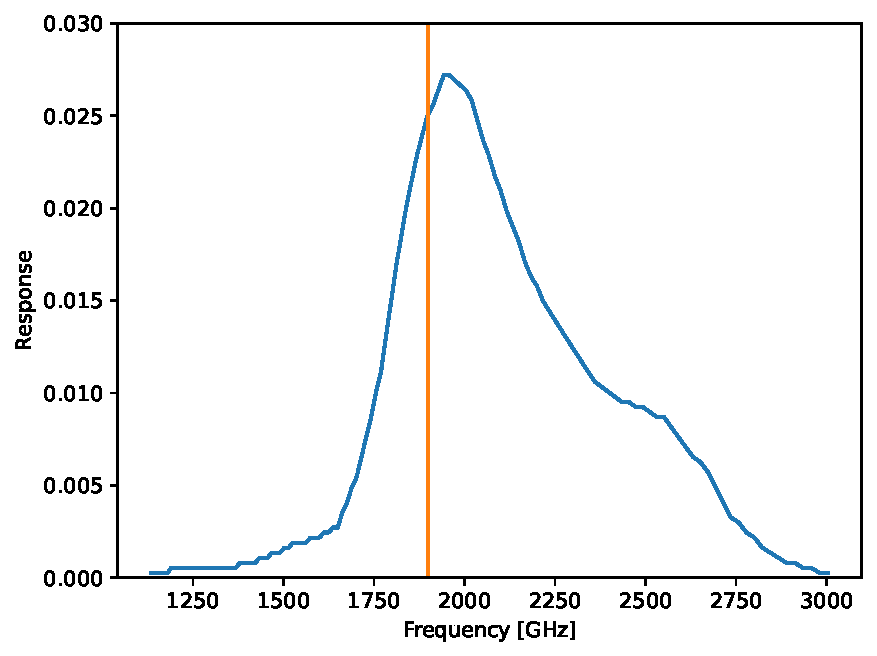
\includegraphics[width=\columnwidth]{figures/dirbe_09_bandpass_vs_cii.pdf}
    \caption{The DIRBE 140 $\mu$ m bandpass profile. The orange vertical line marks the rest frequency of the \cii\ line.}
    \label{fig:140_bp}
\end{figure}

\subsection{FIRAS}
The \COBE-FIRAS experiment was an absolutely calibrated differential Michelson Fourier transform interferometer that observed the full sky from 68\,GHz--2911\,GHz with 13.6\,GHz frequency resolution \citep{fixsen:1994,mather:1999}. 

Although the main goal of FIRAS was the characterization of the CMB blackbody spectrum \citep{mather:1994}, it is also a very important dataset in the determination of emission lines such as \cii, because of its high resolution in frequency space.

In the DR2 analysis, we are using only a subset of the FIRAS frequency bands, listed in \citet{CG02_01}; their usage serves two main purposes: First, since FIRAS was absolutely calibrator, it is an important check on the calibration of other data sets -- here, we use it to contribute to the calibration of the \hfi\ bands, as well as the 100, 140 and 240 $\mu$ m DIRBE bands. Second, as mentioned above, the high frequency resolution of DIRBE means that it is effective in constraining the \cii\ line: By comparing the observed sky at DIRBE band 9 with the FIRAS data roughly around this wavelength, we can see what part of the band 9 radiation which is coming from \cii\ line emission. Thus, the most important FIRAS bands for the present paper are the ones between 1809-2081 GHz, which are used for the \cii\ constraints, as well as the 2135 GHz one, which is used to assist in the calibration of DIRBE band 9, which in turn provides a check on the overall scaling of the resulting \cii\ maps.

\subsection{Other data sets}
As mentioned above, the global analysis of which this paper is a part includes several data sets in order to help constrain the sky model at the frequencies we are considering. In addition to the DIRBE and FIRAS bands not directly impacting this paper, there are two other data sets which are used, which will briefly be mentioned here.

\subsubsection{\Planck\ HFI}
The \Planck\ High Frequency Instrument (HFI; \citealt{planck2016-l03}) observed
the sky in six frequency channels from 100 GHz to 857 GHz, with the primary
purpose being characterizing temperature fluctuations in the CMB to
unprecedentedly small scales. As it also was able to target the far-infrared
sky, it is able to shed light on the dust component in this frequency range.

The importance of HFI for this paper is thus in its ability to constrain the
dust SED and morphology at lower frequencies, which impacts the modelling of
dust at DIRBE band 9 and thus indirectly impacts the quality of the \cii\ maps.

\subsubsection{\Gaia}
The \Gaia\ DR2 \citep{gaia:2016,gaia:2018} and \WISE \citep{wright:2010}
datasets are used to fit point sources that are found in the near-infrared sky.
The impact of such point sources on the \cii\ modelling is expected to be
relatively small, as there are few point sources visiable in the ninth DIRBE
band.


\clearpage
\section{Astrophysical results}

\clearpage
\section{Future directions}

\clearpage
\section{Conclusions}

\begin{figure}
    \centering
    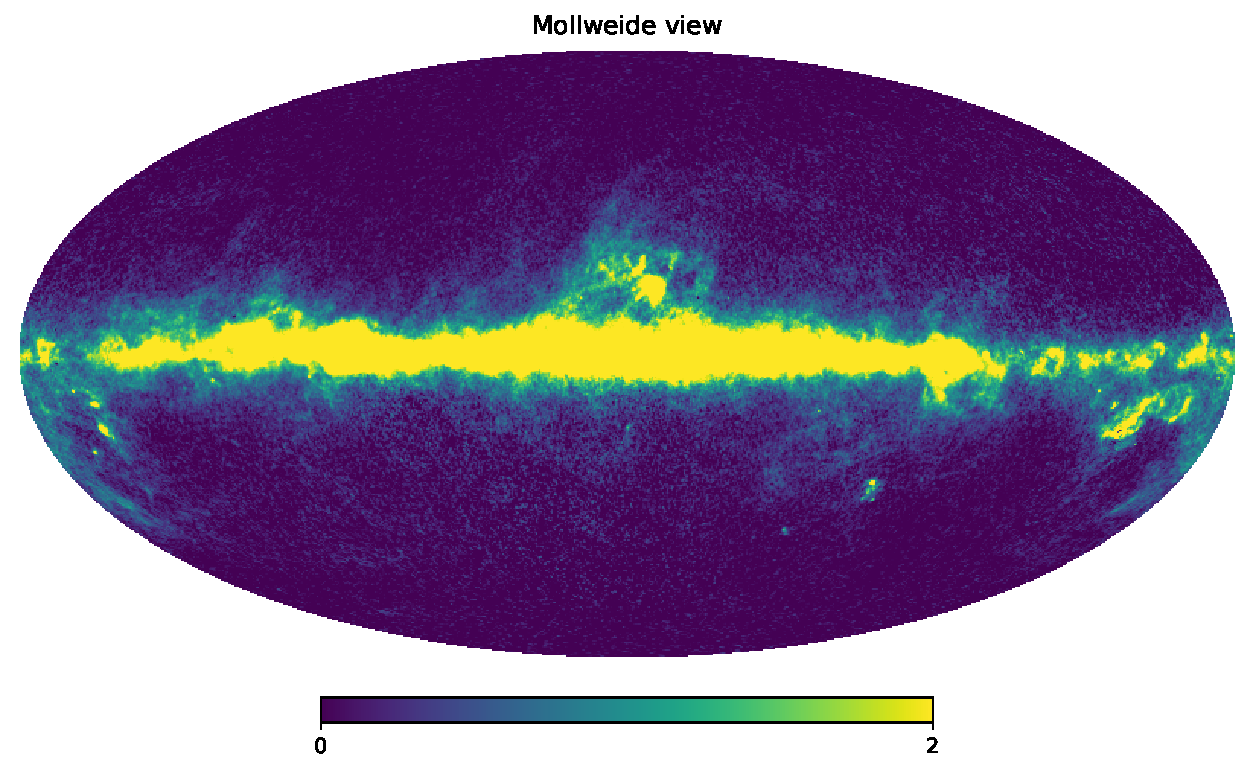
\includegraphics[width=\columnwidth]{figures/cii_meanmap.pdf}
    \caption{The mean over the CII map samples.}
    \label{fig:cii_mean}
\end{figure}

\begin{figure}
    \centering
    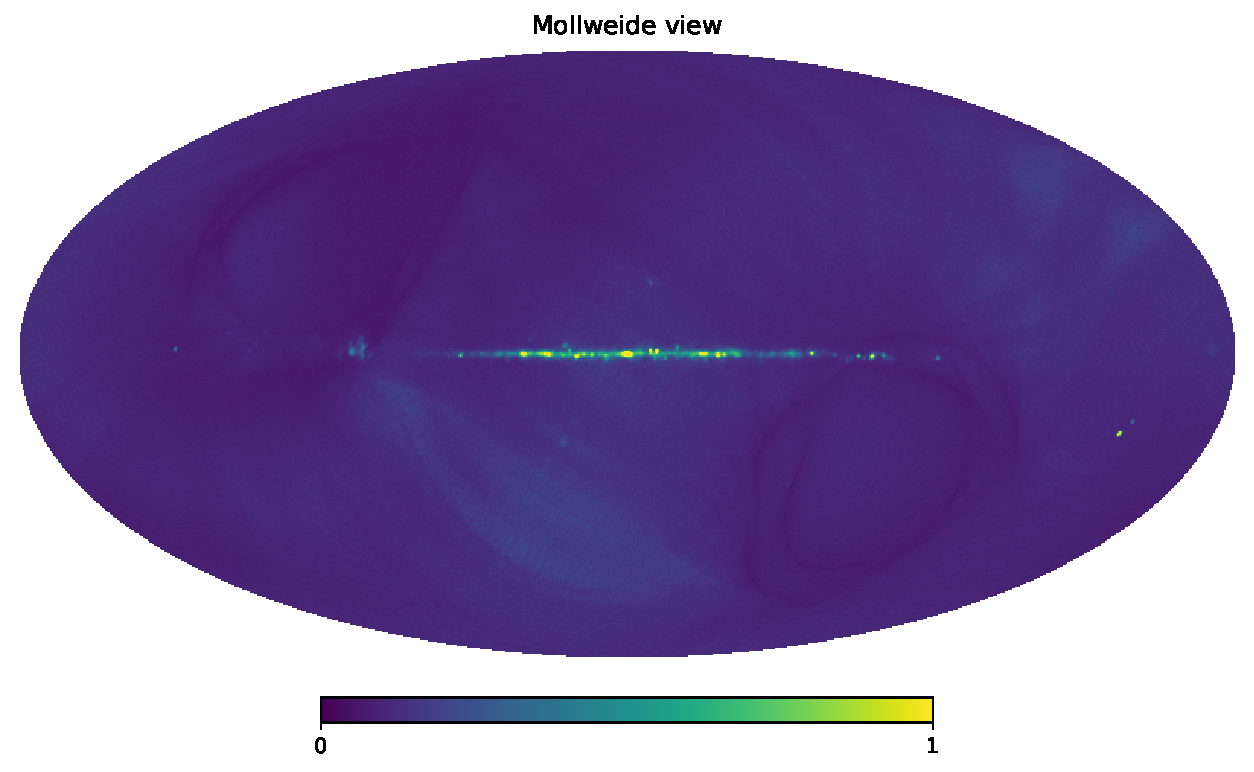
\includegraphics[width=\columnwidth]{figures/cii_stdmap.pdf}
    \caption{The standard deviation of the CII map samples.}
    \label{fig:cii_std}
\end{figure}

\begin{figure}
    \centering
    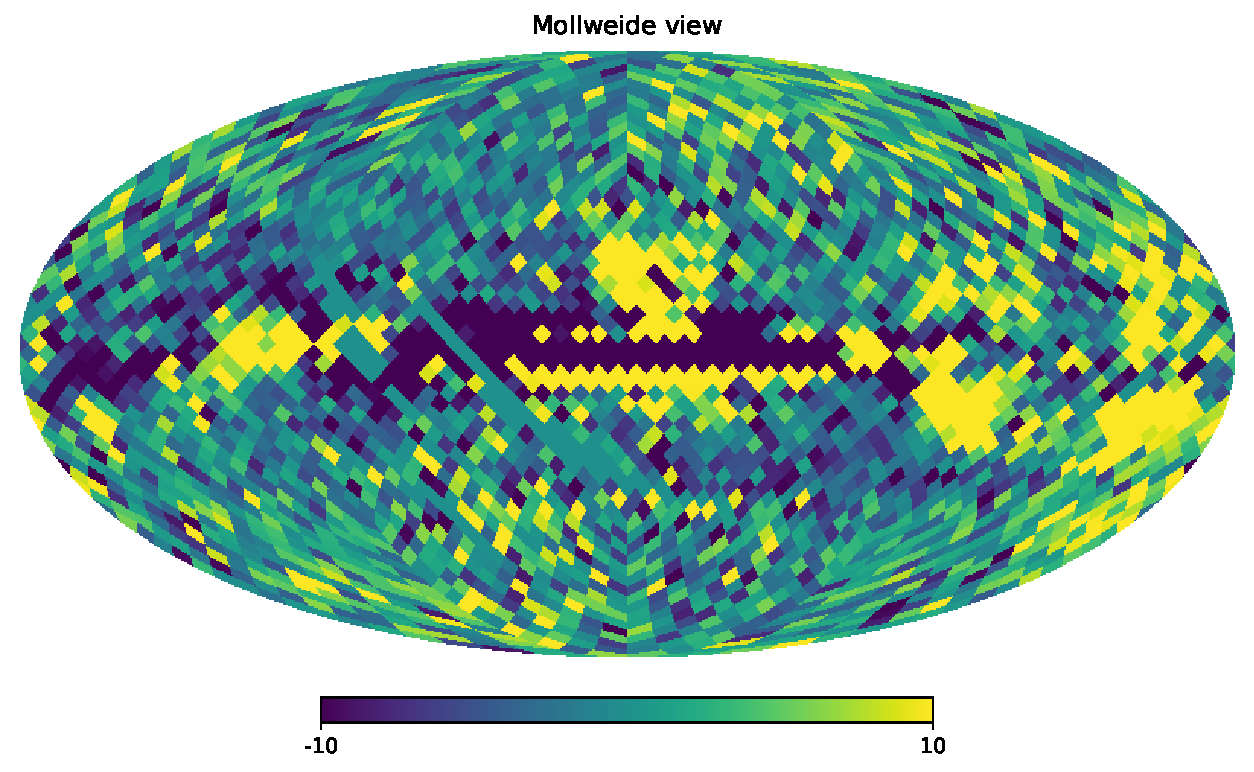
\includegraphics[width=\columnwidth]{figures/res_FIRAS_H1904_c0001_k000700.pdf}
    \caption{The FIRAS 1904 GHz channel residual.}
    \label{fig:firas_1904_res}
\end{figure}

\begin{figure}
    \centering
    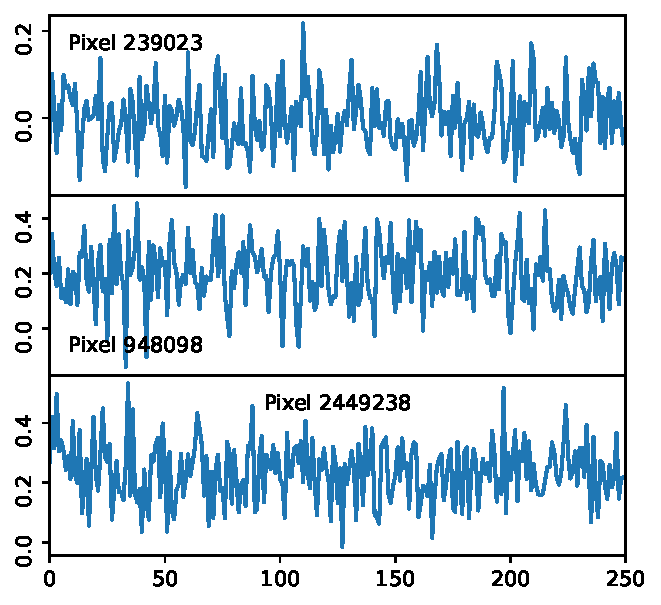
\includegraphics[width=\columnwidth]{figures/traceplots_cii_amps.pdf}
    \caption{Traceplots for the CII amplitudes for three selected pixels.}
    \label{fig:traceplots_cii_amps}
\end{figure}

\begin{figure}
    \centering
    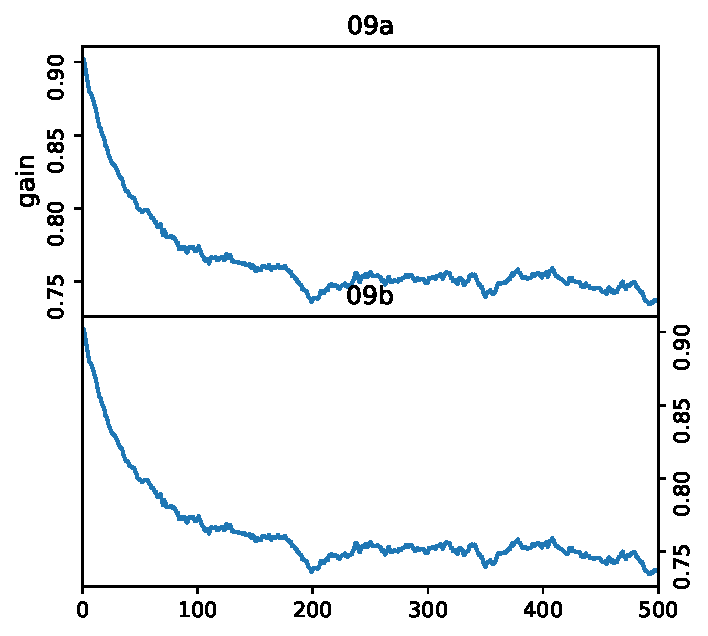
\includegraphics[width=\columnwidth]{figures/traceplots_cii_gains.pdf}
    \caption{Traceplots for the gains of the two 09 DIRBE bands.}
    \label{fig:traceplots_cii_gains}
\end{figure}

\begin{figure}
    \centering
    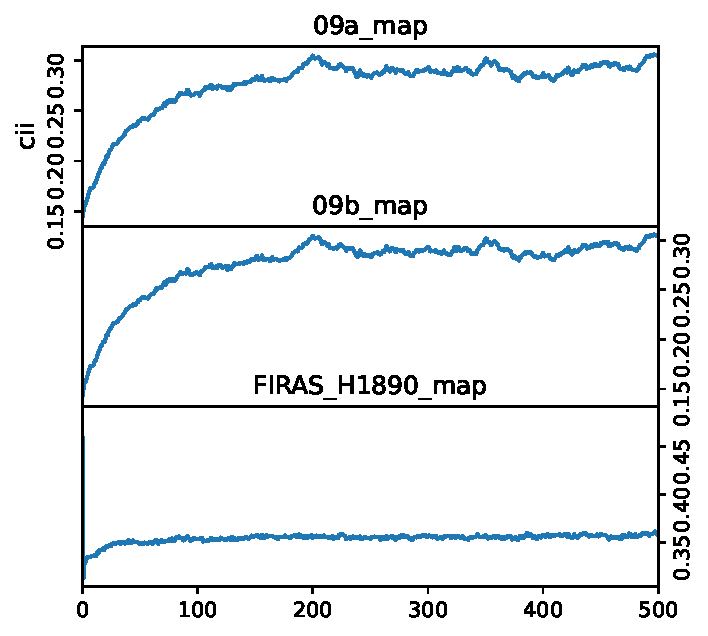
\includegraphics[width=\columnwidth]{figures/traceplots_cii_lineratios.pdf}
    \caption{Traceplots for the line ratios at the two 09 DIRBE bands as well as the 1890 FIRAS band.}
    \label{fig:traceplots_cii_lineratios}
\end{figure}

\begin{figure}
    \centering
    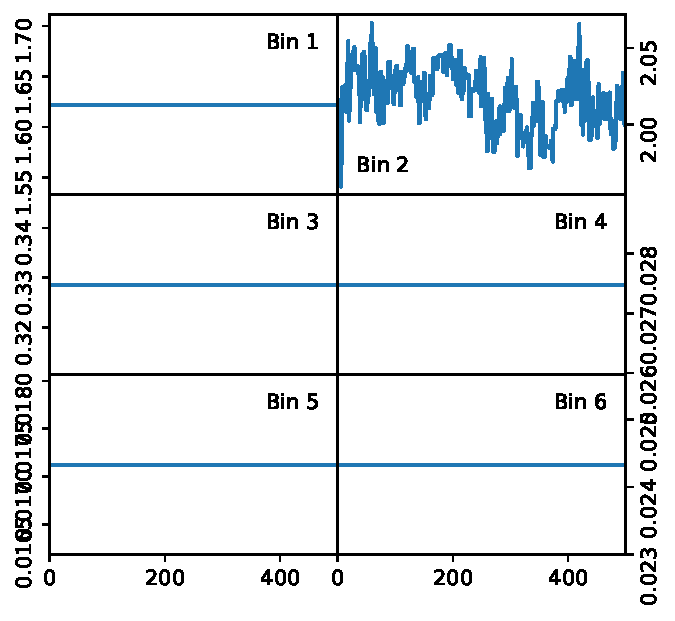
\includegraphics[width=\columnwidth]{"figures/traceplots_dust_seds_cold_dust.pdf"}
    \caption{Traceplots for the dust SEDs for the cold dust component.}
    \label{fig:traceplots_dust_seds_colddust}
\end{figure}

\begin{figure}
    \centering
    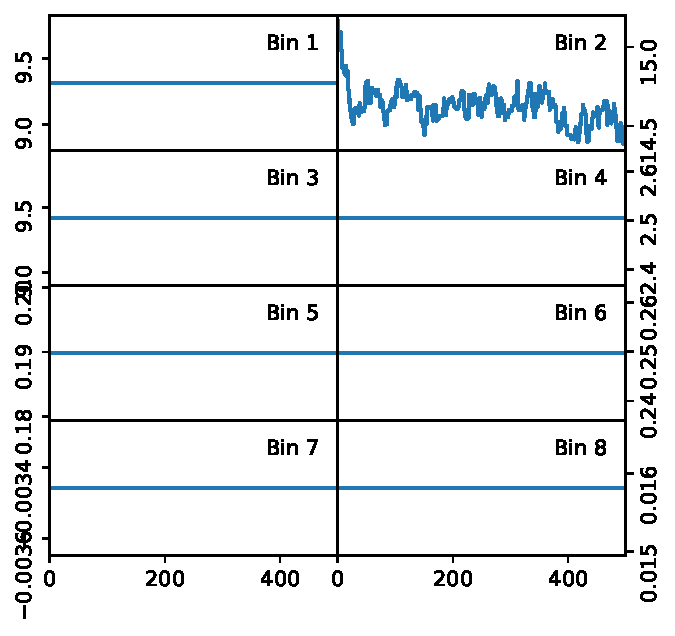
\includegraphics[width=\columnwidth]{"figures/traceplots_dust_seds_hot_dust.pdf"}
    \caption{Traceplots for the dust SEDs for the hot dust component.}
    \label{fig:traceplots_dust_seds_hotdust}
\end{figure}

\begin{figure}
    \centering
    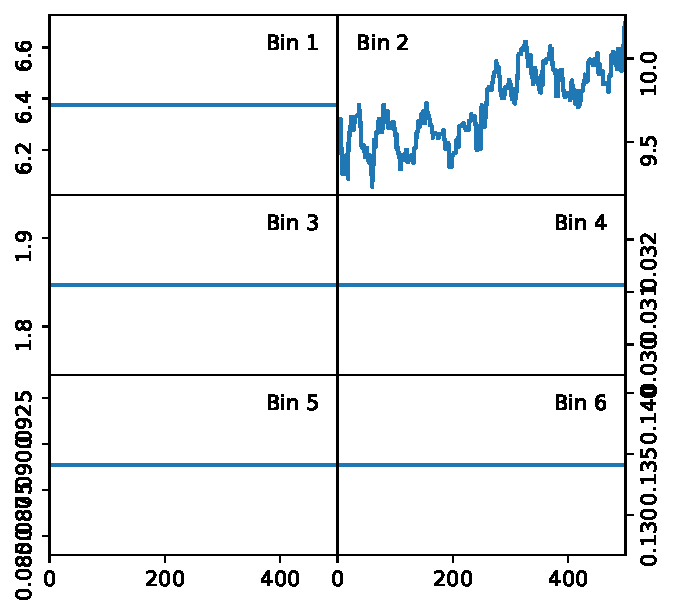
\includegraphics[width=\columnwidth]{"figures/traceplots_dust_seds_nearby_dust.pdf"}
    \caption{Traceplots for the dust SEDs for the nearby dust component.}
    \label{fig:traceplots_dust_seds_nearbydust}
\end{figure}

\begin{figure}
    \centering
    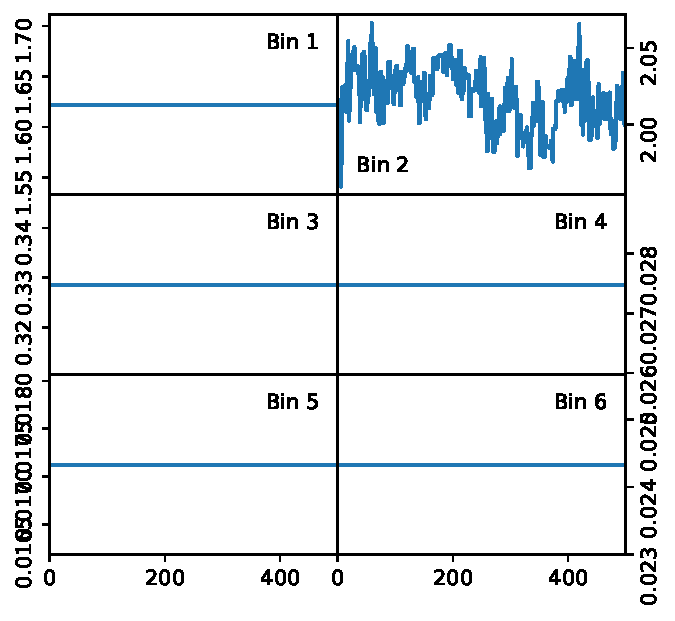
\includegraphics[width=\columnwidth]{"figures/traceplots_dust_sed_slopes_cold_dust.pdf"}
    \caption{Traceplots for the dust SED slopes for the cold dust component.}
    \label{fig:traceplots_dust_sed_slopes_colddust}
\end{figure}

\begin{figure}
    \centering
    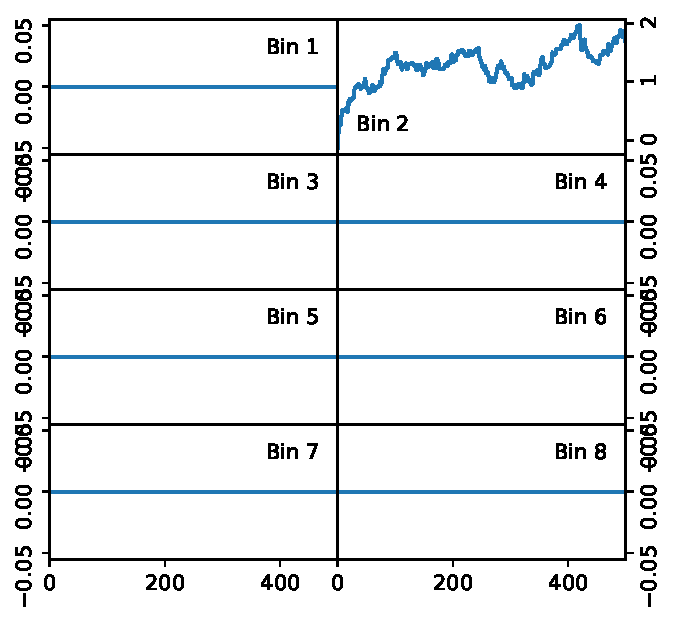
\includegraphics[width=\columnwidth]{"figures/traceplots_dust_sed_slopes_hot_dust.pdf"}
    \caption{Traceplots for the dust SED slopes for the hot dust component.}
    \label{fig:traceplots_dust_sed_slopes_hotdust}
\end{figure}

\begin{figure}
    \centering
    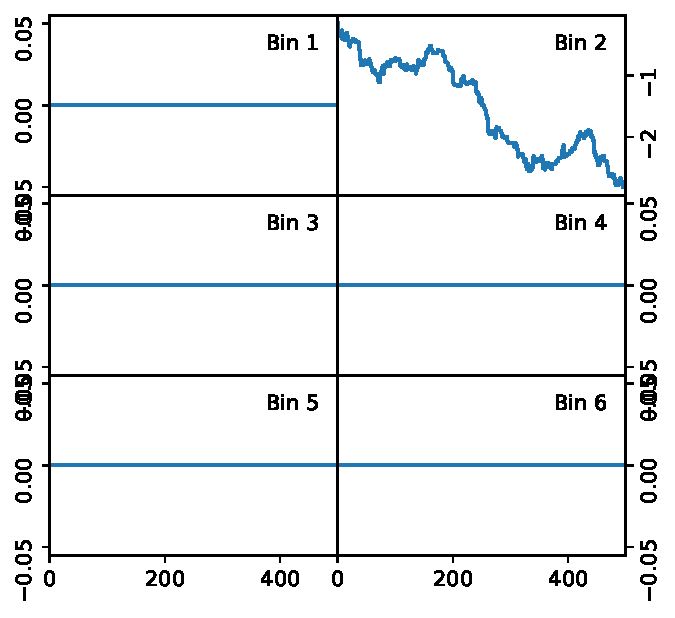
\includegraphics[width=\columnwidth]{"figures/traceplots_dust_sed_slopes_nearby_dust.pdf"}
    \caption{Traceplots for the dust SED slopes for the nearby dust component.}
    \label{fig:traceplots_dust_sed_slopes_nearbydust}
\end{figure}


\blindtext





\begin{acknowledgements}
 The current work has received funding from the European
  Union’s Horizon 2020 research and innovation programme under grant
  agreement numbers 819478 (ERC; \textsc{Cosmoglobe}) and 772253 (ERC;
  \textsc{bits2cosmology}). Some of the results in this paper have been derived using the HEALPix \citep{HEALPIX} package.
  We acknowledge the use of the Legacy Archive for Microwave Background Data
  Analysis (LAMBDA), part of the High Energy Astrophysics Science Archive Center
  (HEASARC). HEASARC/LAMBDA is a service of the Astrophysics Science Division at
  the NASA Goddard Space Flight Center.  
\end{acknowledgements}


%-------------------------------------------------------------
%                                       Table with references 
%-------------------------------------------------------------
%

\bibliographystyle{aa}
\bibliography{../../common/CG_bibliography,references,../../common/Planck_bib}
\end{document}
%%%% End of aa.dem
